% !TeX program = xelatex
\documentclass[12pt]{article}

\usepackage{lab_report}

\title{min-GPT}
\subtitle{Decoder-Only Transformer-based Dialogue Language Model Report}
\author{Yuhang Yang}
\date{2026 年 8 月}
\shortauthor{Y. Yang}
\shorttitle{min-GPT 项目报告}

\newcommand{\EOS}{\mathrm{EOS}}
\newcommand{\Vocab}{\mathcal V}
\newcommand{\RSpace}{\mathbb R}

\begin{document}
\maketitle

\begin{abstract}
本报告完整介绍 min-GPT 项目：一个以 DialoGPT-small 初始化、在 DailyDialog 上进行 fine-tuning、代码可直接阅读的对话式 Decoder-only GPT。项目实现覆盖 GPT-2 byte-level BPE tokenization、对话样本构造、causal multi-head self-attention、GPT-2 权重转换、reply-only supervision，以及 autoregressive 命令行生成；并且报告选取一个真实对话样本，逐步追踪它从英文文本和 UTF-8 bytes，经 pseudo-text、BPE tokens、token IDs、tensors、logits 与 loss，最终到 decoded output 的全部表示过程；同时，报告记录了本项目唯一一次正式训练、完整 held-out test evaluation 与 fixed-prompt generation 结果。
\end{abstract}

\section{项目目标与系统概览}

min-GPT 是一个 end-to-end 对话语言模型项目，其核心机制均直接呈现在源码中。项目从 \texttt{microsoft/DialoGPT-small} 的 pretrained parameters 出发，在英文 DailyDialog 对话数据上进行 full-parameter fine-tuning，并使用手写的 Decoder-only GPT 生成回复，并且模型保留 12-layer GPT-2 small 配置和约 1.24 亿个 trainable parameters。

完整训练路径为
\begin{equation*}
\begin{aligned}
\text{English dialogue}
&\xrightarrow{\text{byte-level BPE}} \text{token IDs}\\
&\xrightarrow{\text{dataset}} (\texttt{input\_ids},\texttt{labels})\\
&\xrightarrow{\text{Decoder-only GPT}} \text{logits}\\
&\xrightarrow{\text{reply-only cross-entropy}} \mathcal L\\
&\xrightarrow{\text{backpropagation + AdamW}} \theta'.
\end{aligned}
\end{equation*}
在 generation 阶段，模型无法获得 ground-truth reply，它从一个 prompt 开始，每次采样并追加一个 token：
\begin{equation}
(p_1,\ldots,p_m)
\longrightarrow \hat y_1
\longrightarrow \hat y_2
\longrightarrow \cdots
\longrightarrow \EOS .
\end{equation}

实现按职责拆分：\texttt{config.py} 保存共享常量；\texttt{tokenizer.py} 完成 text 与 token IDs 之间的转换；\texttt{data.py} 从 history--reply 记录构造训练 tensors；\texttt{model.py} 实现网络并导入 pretrained weights；\texttt{train.py} 优化模型并保存 checkpoints；\texttt{generate.py} 则提供 single-turn generation、interactive chat 与 baseline comparison。

与 encoder--decoder Transformer 不同，本项目没有 encoder memory，也没有 cross-attention。Dialogue history 与 reply 位于同一个 token sequence 中，所有依赖关系均通过序列内部的 causal self-attention 传递。

\section{GPT-2 Byte-Level BPE Tokenizer}

\subsection{固定 vocabulary 与 merge table}

Tokenizer 使用随 DialoGPT-small 发布的 \texttt{vocab.json} 与 \texttt{merges.txt}，Vocabulary 将 token strings 映射为整数 IDs，其固定大小为
\[
|\Vocab|=50257.
\]
Merge file 给出 byte pairs 的优先级顺序，即文件中越早出现的 pair 具有越小的 rank，因而会被 BPE 更早合并。Fine-tuning 不会重建 merge table，也不会增加 vocabulary entries；它更新的是模型中的 continuous embedding vectors，而 tokenizer 的 discrete segmentation rules 保持不变。

初始化过程构造 forward vocabulary、inverse vocabulary、byte bijection、inverse byte bijection、merge ranks 与 cache：
\begin{pythoncode}[label={lst:tokenizer-init}]
self.encoder = vocab
self.decoder = {token_id: token for token, token_id in vocab.items()}
self.byte_encoder = bytes_to_unicode()
self.byte_decoder = {
    char: byte for byte, char in self.byte_encoder.items()
}
self.bpe_ranks = {pair: rank for rank, pair in enumerate(merges)}
self.cache = {}
\end{pythoncode}
这里的 \texttt{encoder} 与 \texttt{decoder} 只是普通 dictionaries，与原始 Transformer architecture 中的 encoder 和 decoder modules 无关。

\subsection{支持 Unicode 的 pre-tokenization}

GPT-2 在执行 BPE 之前先用 regular expression 将文本切分为较粗粒度的 pieces。Python 标准 \texttt{re} module 并不直接实现 Unicode properties \texttt{\textbackslash p\{L\}} 与 \texttt{\textbackslash p\{N\}}，因此本项目遍历全部 Unicode code points，调用 \texttt{unicodedata.category()}，动态构造 letters 与 numbers 的 character ranges。

最终 expression 可以识别 \texttt{'s}、\texttt{'re}、\texttt{'ll} 等 contractions；可能带一个 leading space 的 letter 与 number sequences；punctuation 及其他 non-whitespace symbols；以及 whitespace sequences。空格通常会与其后的单词分在一起，例如，\texttt{``You know''} 首先被切分为 \texttt{``You''} 和 \texttt{`` know''}，后者随后在 GPT-2 pseudo-text 中表示为 \texttt{\string Ġknow}。

\subsection{UTF-8 bytes 与 pseudo-text characters}

Byte-level BPE 并不直接合并原始 Unicode code points，而是先将每个 pre-tokenized piece 转换为 UTF-8 bytes。一个 byte 只有 256 种可能取值，但其中许多值不可打印，因此函数 \texttt{bytes\_to\_unicode()} 构造如下 bijection：
\begin{equation}
b\in\{0,\ldots,255\}
\xleftrightarrow{\text{bijection}}
c_b\in\mathcal C_{\mathrm{BPE}}.
\end{equation}
$\mathcal C_{\mathrm{BPE}}$ 中的 characters 是 merge algorithm 的中间载体，本文将其称为 \emph{pseudo-text}：它们看起来像普通字符，但用途是以可逆方式表示 bytes。

转换过程实现如下：
\begin{pythoncode}[label={lst:byte-encode}]
for word in TOKEN_PATTERN.findall(text):
    byte_text = "".join(
        self.byte_encoder[byte]
        for byte in word.encode("utf-8")
    )
    tokens.extend(self.bpe(byte_text))
\end{pythoncode}
常见 ASCII letters 映射为自身，而 space byte 映射为 \texttt{\string Ġ}，因此，\texttt{`` fitness''} 会以 \texttt{\string Ġfitness} 的形式参与 BPE，最终显示的 reply 不会包含字面上的 \texttt{\string Ġ}，因为 decoding 会将其还原为原始 space byte。

\subsection{BPE merge algorithm}

Let the mapped characters of one piece be
\[
w=(c_1,c_2,\ldots,c_n).
\]
每轮迭代枚举相邻 pairs
\[
\mathcal P(w)=\{(c_1,c_2),(c_2,c_3),\ldots,(c_{n-1},c_n)\}
\]
并选择已记录 rank 最小的 pair：
\begin{equation}
p^*=\arg\min_{p\in\mathcal P(w)}\operatorname{rank}(p).
\end{equation}
若 $p^*$ 不在 merge table 中，过程停止；否则合并该 pair 的所有相邻出现位置，并继续检查新的 sequence。

\begin{pythoncode}[label={lst:bpe-loop}]
while len(word) > 1:
    pairs = set(zip(word, word[1:]))
    pair = min(
        pairs,
        key=lambda item: self.bpe_ranks.get(item, float("inf")),
    )
    if pair not in self.bpe_ranks:
        break
    word = merge_all_occurrences(word, pair)
\end{pythoncode}
实际源码直接在 loop 内完成 merge scan，并且由于同一个 piece 可能重复出现，最终 token list 会缓存在 \texttt{self.cache} 中。

\subsection{Encode、decode 与 EOS}

完整 encode 路径为
\begin{equation}
\text{text}
\rightarrow \text{UTF-8 bytes}
\rightarrow \text{pseudo-text}
\rightarrow \text{BPE tokens}
\rightarrow \text{token IDs}.
\end{equation}
Decoding 执行相反的操作：
\begin{equation}
\text{token IDs}
\rightarrow \text{token strings}
\rightarrow \text{pseudo-text}
\rightarrow \text{bytes}
\rightarrow \text{UTF-8 text}.
\end{equation}

\begin{pythoncode}[label={lst:decode}]
byte_text = "".join(tokens)
byte_values = bytes(
    self.byte_decoder[char] for char in byte_text
)
return byte_values.decode("utf-8", errors="replace")
\end{pythoncode}

Special token \texttt{<|endoftext|>} 的 ID 为
\[
\texttt{EOS\_ID}=50{,}256.
\]
它用于分隔 utterances、标记 supervised reply 的结束位置，并告诉 generation 何时停止。当 \texttt{skip\_special\_tokens=True} 时，\texttt{decode()} 会在重建 byte sequence 前移除该 ID；否则它会还原为字面字符串 \texttt{<|endoftext|>}。

\section{DailyDialog 数据表示与加载}

\subsection{最终磁盘格式}

文件 \texttt{train.txt}、\texttt{validation.txt} 与 \texttt{test.txt} 保存英文对话数据，虽然扩展名为 \texttt{.txt}，单每个文件实际采用 JSON Lines：每个非空行都是可以独立解析的 JSON object。
\begin{verbatim}
{"history":["...", "..."],"reply":"..."}
\end{verbatim}
\texttt{history} 是 target 之前按顺序排列的 utterance list，\texttt{reply} 则是需要监督的 next utterance。加载逻辑刻意保持简洁：
\begin{pythoncode}[label={lst:data-load}]
path = Path(data_dir) / f"{split}.txt"
with open(path, encoding="utf-8") as file:
    self.data = [
        json.loads(line) for line in file if line.strip()
    ]
\end{pythoncode}

最终 split sizes 见表~\ref{tab:data-size}。
\begin{table}[htbp]
\centering
\caption{DailyDialog next-utterance 样本数量}
\label{tab:data-size}
\begin{tabular}{lr}
\toprule
Split & 样本数\\
\midrule
Train & 76,052\\
Validation & 7,069\\
Test & 6,740\\
\bottomrule
\end{tabular}
\end{table}

\subsection{贯穿全文的一个真实样本}

第一条 training record 为
\begin{verbatim}
history:
Say , Jim , how about going for a few beers after dinner ?

reply:
You know that is tempting but is really not good for our fitness .
\end{verbatim}
History 转换为以下 BPE token strings：
\begin{equation*}
\begin{aligned}
(&\texttt{Say},\texttt{\string Ġ,},\texttt{\string ĠJim},\texttt{\string Ġ,},
\texttt{\string Ġhow},\texttt{\string Ġabout},\texttt{\string Ġgoing},
\texttt{\string Ġfor},\texttt{\string Ġa},\texttt{\string Ġfew},\\
&\texttt{\string Ġbeers},\texttt{\string Ġafter},\texttt{\string Ġdinner},
\texttt{\string Ġ?}).
\end{aligned}
\end{equation*}
对应 IDs 为
\begin{equation}
(25515,837,5395,837,703,546,1016,329,257,1178,16800,706,8073,5633).
\end{equation}
Reply IDs 为
\begin{equation}
(1639,760,326,318,29850,475,318,1107,407,922,329,674,13547,764).
\end{equation}
在两侧分别追加 EOS 后，最终 sequence 为
\begin{equation}
X=(\underbrace{h_1,\ldots,h_{14},50256}_{\text{history}},
\underbrace{r_1,\ldots,r_{14},50256}_{\text{reply}}),
\qquad |X|=30.
\end{equation}

\subsection{Reply-first truncation 与完整轮次 history 保留}

Dataset 首先 tokenizes reply 并追加 EOS，若 reply 本身已经超过 256-token context，则将其截断到 256 个位置，并强制把最后一个位置设为 EOS：
\begin{pythoncode}[label={lst:reply-truncate}]
reply = self.tokenizer.encode(sample["reply"]) + eos
if len(reply) > self.context_length:
    reply = reply[: self.context_length]
    reply[-1] = self.tokenizer.eos_token_id
\end{pythoncode}

若仍有空间，则按照从新到旧的顺序检查 history utterances，只有整个 utterance 连同 EOS 都能放入时才予以保留；一旦下一个更早的 turn 无法完整放入，遍历立即停止：
\begin{pythoncode}[label={lst:history-truncate}]
history = []
for text in reversed(sample["history"]):
    utterance = self.tokenizer.encode(text) + eos
    if len(utterance) + len(history) + len(reply) > self.context_length:
        break
    history = utterance + history
\end{pythoncode}
该策略保护完整的 target reply，并使 recent context 优先于 distant context，同时避免旧 utterance 的残缺片段出现在 sample 开头。

\subsection{Reply-only labels 与 batch padding}

单个 item 返回
\begin{equation}
\begin{aligned}
\texttt{input\_ids}&=\text{history}+\text{reply},\\
\texttt{labels}&=(-100,\ldots,-100)+\text{reply IDs}.
\end{aligned}
\end{equation}
对于上述 sample，前 15 个 labels 为 $-100$，后 15 个 labels 包含 reply 及其 EOS：
\begin{equation}
Y=(\underbrace{-100,\ldots,-100}_{15},1639,760,\ldots,13547,764,50256).
\end{equation}

各 sequence 长度不同，当 batch size 为 $B=2$ 时，\texttt{collate\_examples()} 将它们 pad 到该 batch 的最长 sequence：
\[
\texttt{input\_ids},\texttt{labels}\in\mathbb N^{B\times T},
\qquad T\leq256.
\]
Input IDs 在右侧用 EOS padding，labels 则在右侧用 $-100$ padding：
\begin{pythoncode}[label={lst:collate}]
input_ids = torch.full(
    (len(examples), max_length), EOS_ID, dtype=torch.long
)
labels = torch.full(
    (len(examples), max_length), -100, dtype=torch.long
)
\end{pythoncode}
因此，padding 不会贡献 cross-entropy，同时也无需向固定的 GPT-2 vocabulary 引入额外 pad token。

\section{Decoder-Only GPT 模型}

\subsection{配置与 parameter count}

该手写模型在结构上与 GPT-2 small 和 DialoGPT-small 兼容，由于 language-model head 与 token embedding 共享同一个 weight matrix，parameter count 中只计算一次 $50{,}257\times768$ vocabulary matrix：
\begin{equation}
50{,}257\times768+1{,}024\times768
+12\times7{,}087{,}872+1{,}536
=124{,}439{,}808.
\end{equation}
\begin{table}[htbp]
\centering
\caption{Decoder-only GPT 配置}
\label{tab:model-config}
\begin{tabular}{lr}
\toprule
项目 & 数值\\
\midrule
Vocabulary size & 50,257\\
Maximum positions & 1,024\\
Training context & 256\\
Layers & 12\\
Hidden size & 768\\
Attention heads & 12\\
Head size & 64\\
MLP hidden size & 3,072\\
Dropout & 0.1\\
LayerNorm epsilon & $10^{-5}$\\
Trainable parameters & 124,439,808\\
\bottomrule
\end{tabular}
\end{table}

\subsection{Token 与 position embeddings}

Input IDs 的 shape 为
\[
X\in\mathbb N^{B\times T}.
\]
Token table 与 learned position table 分别为
\[
W_{\mathrm{te}}\in\RSpace^{50{,}257\times768},
\qquad
W_{\mathrm{pe}}\in\RSpace^{1{,}024\times768}.
\]
经过 lookup 与 addition 得到
\begin{equation}
H^{(0)}=W_{\mathrm{te}}[X]+W_{\mathrm{pe}}[0:T],
\qquad H^{(0)}\in\RSpace^{B\times T\times768}.
\end{equation}
这些 positions 是 learned parameters，而不是 sinusoidal encodings。

\subsection{Joint QKV projection 与 multi-head reshape}

对于 block input
\[
H\in\RSpace^{B\times T\times C},\qquad C=768,
\]
一个 linear layer 同时计算三组 projections：
\begin{equation}
[Q\ K\ V]=HW_{\mathrm{qkv}}+b_{\mathrm{qkv}}
\in\RSpace^{B\times T\times3C}.
\end{equation}
最后一个维度被拆分为三个 tensors，随后分别执行 reshape 与 transpose：
\begin{pythoncode}[label={lst:qkv}]
batch, length, channels = x.shape
q, k, v = self.c_attn(x).split(channels, dim=2)

q = q.view(batch, length, self.n_head, self.head_size)
q = q.transpose(1, 2)
\end{pythoncode}
由于 $768=12\times64$，最终 shapes 为
\[
Q,K,V\in\RSpace^{B\times12\times T\times64}.
\]
Reshape 只重新组织 tensor axes，而不同 heads 使用 joint \texttt{c\_attn} weights 中不同的 slices，因此能够学习不同 projections。

\subsection{Scaled dot-product attention 与 causal mask}

每个 head 计算
\begin{equation}
S=\frac{QK^\top}{\sqrt{64}},
\qquad S\in\RSpace^{B\times12\times T\times T}.
\end{equation}
除以 $\sqrt{64}$ 可以避免 dot-product magnitude 随 head dimension 增长，从而防止 softmax 进入过度饱和区域。

Decoder-only model 必须阻止位置 $i$ 读取任意 future position $j>i$，因此每个 attention layer 都注册一个 lower-triangular Boolean buffer：
\begin{pythoncode}[label={lst:causal-buffer}]
mask = torch.tril(
    torch.ones(n_positions, n_positions, dtype=torch.bool)
)
self.register_buffer(
    "bias", mask.view(1, 1, n_positions, n_positions)
)
\end{pythoncode}
当 $T=4$ 时，可见性矩阵为
\[
M=\begin{pmatrix}
1&0&0&0\\
1&1&0&0\\
1&1&1&0\\
1&1&1&1
\end{pmatrix}.
\]
\texttt{register\_buffer} 将 mask 纳入 model state，使其随 \texttt{model.to(device)} 一同移动，但不会将其变为 trainable parameter，存储 shape 为 $(1,1,1024,1024)$；forward pass 截取 $(1,1,T,T)$，再沿 batches 与 heads 广播。

Future scores 被设为 $-\infty$：
\begin{equation}
\widetilde S_{ij}=\begin{cases}
S_{ij},&j\leq i,\\
-\infty,&j>i.
\end{cases}
\end{equation}
因此，$A=\operatorname{softmax}(\widetilde S)$ 为 future positions 分配的 probability 严格为零。

\subsection{Value aggregation 与 head merging}

每个 head 对 values 进行加权求和，
\begin{equation}
O_h=A_hV_h\in\RSpace^{B\times T\times64}.
\end{equation}
随后将 12 个 heads 重新拼接为 $(B,T,768)$，并通过 output projection：
\begin{pythoncode}[label={lst:attention-output}]
weights = self.attn_dropout(torch.softmax(scores, dim=-1))
output = weights @ v
output = output.transpose(1, 2).contiguous()
output = output.view(batch, length, channels)
return self.resid_dropout(self.c_proj(output))
\end{pythoncode}

\subsection{Pre-LayerNorm blocks 与 GELU-new MLP}

每个 block 都采用 Pre-LayerNorm residual updates：
\begin{equation}
\begin{aligned}
H'&=H+\operatorname{Attention}(\operatorname{LN}_1(H)),\\
H_{\mathrm{out}}&=H'+\operatorname{MLP}(\operatorname{LN}_2(H')).
\end{aligned}
\end{equation}
LayerNorm 位于每个 sub-layer 之前，从而在 attention 与 MLP 外侧保留直接的 residual path。

MLP 将最后一个维度从 768 扩展到 3072，并应用 GPT-2 的 GELU-new activation：
\begin{equation}
\operatorname{GELU}_{\mathrm{new}}(x)
=\frac12x\left[1+\tanh\left(\sqrt{\frac2\pi}
(x+0.044715x^3)\right)\right].
\end{equation}
第二个 linear layer 再将其投影回 768，随后执行 dropout。

\subsection{Layer stack、final normalization 与 weight tying}

12 个 blocks 始终保持 representation shape：
\[
H^{(0)}\rightarrow H^{(1)}\rightarrow\cdots\rightarrow H^{(12)},
\qquad H^{(l)}\in\RSpace^{B\times T\times768}.
\]
Final LayerNorm 与 language-model head 输出
\begin{equation}
Z=\operatorname{LN}_f(H^{(12)})W_{\mathrm{lm}}^\top,
\qquad Z\in\RSpace^{B\times T\times50{,}257}.
\end{equation}
源码设置
\[
W_{\mathrm{lm}}=W_{\mathrm{te}},
\]
因此，input embedding 与 output vocabulary classifier 实际指向同一个 parameter object，这就是 weight tying。

\section{导入 DialoGPT-small Weights}

在从以下路径载入 pretrained tensors 之后，上述 architecture 就处于预训练模型状态：
\begin{center}
\nolinkurl{.cache/DialoGPT-small/model.safetensors}
\end{center}


Hugging Face GPT-2 使用 \texttt{Conv1D} class 表示 projections，其 weight layout 相对于 \texttt{torch.nn.Linear} 是转置的，从而受影响的 tensors 包括 attention input/output weights 与两个 MLP projection weights，导入 loop 通过以下 suffixes 识别它们：
\begin{pythoncode}[label={lst:weight-import}]
for name, parameter in model.named_parameters():
    value = weights[name]
    if name.endswith((
        "c_attn.weight", "c_fc.weight", "c_proj.weight"
    )):
        value = value.t()
    parameter.copy_(value.float())
\end{pythoncode}
Embeddings、LayerNorm parameters 与 biases 无需转置即可复制，所有 tensors 先在 CPU 上加载、转换为 FP32，再复制进手写模型，因此，fine-tuning 从英文对话语言模型而非 random weights 开始；DailyDialog 则使该 pretrained model 适应日常 next-utterance responses 的数据分布。

\section{Fine-Tuning 机制}

\subsection{Next-token shift 与 reply-only loss}

Forward pass 返回
\[
Z\in\RSpace^{B\times T\times|\Vocab|}.
\]
位置 $t$ 的 logits 用于预测位置 $t+1$ 的 token，实现中将 logits 与 labels 向相反方向 shift：
\begin{pythoncode}[label={lst:loss-shift}]
logits = model(input_ids)
loss = F.cross_entropy(
    logits[:, :-1].reshape(-1, logits.size(-1)),
    labels[:, 1:].reshape(-1),
    ignore_index=-100,
)
\end{pythoncode}
若 $\mathcal R$ 表示 supervised reply positions 的集合，则 objective 为
\begin{equation}
\mathcal L=-\frac1{|\mathcal R|}
\sum_{t\in\mathcal R}
\log p_\theta(y_t\mid x_1,\ldots,x_{t-1}).
\end{equation}
History labels 为 $-100$，但 history tokens 仍保留在 \texttt{input\_ids} 中。Reply positions 可以 attend to 它们，reply loss gradients 也会沿这些 attention paths 传播。数值 $-100$ 只会将对应位置排除在 direct loss supervision 之外，并不会将该位置从 model input 中移除。

\subsection{Gradient accumulation 与 effective batch size}

Micro-batch size 为 2，accumulation count 为 16，因此 effective batch 为
\[
2\times16=32
\]
个 dialogue examples / optimizer update。每个 micro-batch loss 在 backpropagation 前除以 16：
\begin{equation}
g=\sum_{i=1}^{16}\nabla_\theta\frac{\mathcal L_i}{16}.
\end{equation}
Optimizer 在 accumulation 期间不会执行 step，这样既能保留较大的 effective batch，又能使每次 forward/backward pass 足够小，从而适应可用 device memory。

\subsection{AdamW 与 gradient clipping}

全部 model parameters 均交由 AdamW 优化，weight decay 为 $\lambda=0.01$：
\[
\theta_{s+1}=\operatorname{AdamW}(\theta_s,g_s,\eta_s,\lambda).
\]
当前实现仅使用一个 optimizer parameter group，因此 matrices、biases、LayerNorm parameters 与 embeddings 使用相同的 weight decay。

每次 optimizer step 之前，global gradient norm 都会被 clip 到 1.0。Norm clipping 不改变足够小的 gradients，只对异常大的 gradients 重新缩放，从而降低突发更新破坏 pretrained representations 的风险。

\subsection{Warmup 与 cosine learning-rate decay}

唯一一次正式训练配置为 2500 个 optimizer steps。前 100 steps 采用 linear warmup 达到 peak learning rate，其余部分按照 cosine decay 降至 minimum：
\begin{equation}
\eta_s=
\begin{cases}
\eta_{\max}\dfrac{s}{100},&1\leq s\leq100,\\[6pt]
\eta_{\min}+\dfrac12(\eta_{\max}-\eta_{\min})
\left[1+\cos\left(\pi\dfrac{s-100}{2500-100}\right)\right],
&100<s\leq2500,
\end{cases}
\end{equation}
where
\[
\eta_{\max}=2\times10^{-5},
\qquad
\eta_{\min}=2\times10^{-6}.
\]
Warmup 限制训练初期对 pretrained parameters 的扰动，cosine decay 则在训练后期逐渐减小更新幅度。

\subsection{Device selection、validation 与 checkpoints}

Device priority 为
\[
\mathrm{MPS}\rightarrow\mathrm{CUDA}\rightarrow\mathrm{CPU}.
\]
若 Apple MPS 可用则优先选择；否则依次检查 NVIDIA CUDA 与 CPU。

首次 update 之前，step 0 先测量 baseline validation loss，此后每 50 个 optimizer steps，evaluation 处理固定的前 20 个 deterministic validation batches，并计算以 reply token 加权的 mean：
\begin{equation}
\mathcal L_{\mathrm{val}}
=\frac{\sum\text{valid reply-token losses}}
{\sum\text{valid reply tokens}},
\qquad
\operatorname{PPL}=\exp(\mathcal L_{\mathrm{val}}).
\end{equation}

\texttt{latest.pt} 保存最近的 validation point，而 \texttt{best.pt} 只在 validation loss 达到新的 minimum 时覆盖。每个 checkpoint 包含 model state dictionary、optimizer step 与对应 validation loss。Weights \& Biases 记录该 run 的 training loss、learning rate、gradient norm、validation loss 与 perplexity。

\section{Autoregressive Generation}

\subsection{Prompt representation 与 history trimming}

Single-turn prompt 经过 tokenization 后以 EOS 结尾。若 prompt 过长，则只保留最后 255 个 content tokens，再追加 EOS，使 input tokens 最多为 256 个。Interactive chat 将每条 user utterance 与 model reply 表示为一个以 EOS 结束的 turn。当累计 history 过长时，优先删除最旧的完整 turns。

\subsection{采样一个 next token}

在 generation step $t$，设当前 sequence 为
\[
X^{(t)}=(p_1,\ldots,p_m,\hat y_1,\ldots,\hat y_{t-1}).
\]
Forward pass 为每个 input position 返回 logits，但 generation 只使用最后一个 vector：
\[
z^{(t)}=Z_{-1,:}\in\RSpace^{50{,}257}.
\]

首先，对 context 中已经出现的每个 token 应用 repetition penalty $r=1.1$：positive logits 除以 $r$，negative logits 乘以 $r$，这一 sign-aware operation 在两种情况下都会降低 repeated tokens 的相对 probability，随后使用 temperature $\tau=0.75$ 对 logits 重新缩放：
\[
\widetilde z_v=\frac{z_v}{\tau}.
\]
由于 $\tau<1$，distribution 会更加集中，仅保留最大的 $k=50$ 个 logits，并使用固定 CPU generator 执行 multinomial sampling：
\begin{pythoncode}[label={lst:sampling}]
top_logits, top_indices = torch.topk(logits, k)
probabilities = torch.softmax(top_logits, dim=-1)
sampled = torch.multinomial(
    probabilities, 1, generator=generator
)
next_id = top_indices[sampled].item()
\end{pythoncode}
若 \texttt{next\_id == EOS\_ID}，generation 停止，且 EOS 不会加入 visible suffix；否则追加该 token 并再次运行模型，最多生成 50 个 new tokens。

\subsection{Suffix-only decoding 与 CLI modes}

Generator 单独保存 newly sampled IDs，并且只 decode 这一 suffix，因此不会把 prompt 当作 model reply 的一部分展示。Command-line interface 提供三种 modes：
\begin{itemize}
  \item \texttt{generate}：为单个 prompt 生成一条 reply；
  \item \texttt{chat}：维持简短的 multi-turn terminal conversation；
  \item \texttt{compare}：使用相同的 prompt、seed 与 sampling parameters，对 pretrained baseline 和 fine-tuned model 进行采样比较。
\end{itemize}

当前实现没有 KV cache，每个 generation step 都会将最近 256 个 tokens 重新送入全部 12 layers，并重新计算先前的 keys 与 values，因此该方法必然比 cached decoding 更慢，但能保持 implementation 与 tensor flow 的直接性。

\section{一个 Training Example 的 end-to-end 追踪}

前文引入的真实 DailyDialog sample 按照以下过程通过完整系统。
\begin{enumerate}
  \item Data loader 读取一个 dictionary，其中包含一条 history utterance 与一条 target reply。
  \item Tokenizer 将 text 转换为 UTF-8 bytes，再把 bytes 映射为包含 \texttt{\string Ġ} 等标记的可逆 pseudo-text。
  \item BPE 按照 merge rank 反复合并 pairs，随后 vocabulary lookup 得到 14 个 history IDs 与 14 个 reply IDs。
  \item 在 history 和 reply 后分别追加 EOS ID 50256，得到 30 个 \texttt{input\_ids}。
  \item 前 15 个 labels 变为 $-100$；后 15 个 labels 保留 reply IDs 与 reply EOS。
  \item Collation 将 batch pad 到其最大长度 $T\leq256$，生成两个 $(B,T)$ tensors。
  \item Token embeddings 与 position embeddings 将 IDs 转换为 $(B,T,768)$ continuous representations。
  \item 每一 layer 将其投影为 $(B,12,T,64)$ 的 queries、keys 与 values，计算 $(B,12,T,T)$ causal attention，并沿 attention、MLP 与 residual paths 更新 representation。
  \item 经过 12 layers 后，模型生成 $(B,T,50257)$ logits。
  \item 为进行 next-token alignment，移除最后一个 logit position 与第一个 label position。Cross-entropy 只保留 shift 后不等于 $-100$ 的 labels。
  \item 16 组缩放后的 micro-batch gradients 完成累积；其 global norm 被 clip；AdamW 更新全部 parameters。
  \item Inference 阶段不提供真实 reply，所以 Sampling 从 history 加 EOS 开始，每次生成一个 token，直到遇到 EOS 或达到 50 个 new tokens。
  \item Generated IDs 依次还原为 token strings、pseudo-text、bytes，最终得到显示的英文 reply。
\end{enumerate}

核心区别在于：training 包含完整 reply tensor，并利用 causal mask 并行预测所有 reply positions；generation 阶段尚不存在 future reply tokens，因此 decoding 必须保持 sequential。

\section{最终 Training 与 Evaluation 结果}

\subsection{Training convergence}

唯一一次正式 training run 完成了全部 2500 个 optimizer steps。表~\ref{tab:training-results} 汇总了具有代表性的 monitoring points，这些数值来自固定的前 20 个 validation batches，在 batch size 为 2 时对应 40 条 dialogue samples，它们适合用于一致地比较 checkpoints，但不能视为对完整 validation set 的估计。

\begin{table}[htbp]
\centering
\caption{Fine-tuning 过程中的 reply-only monitoring loss}
\label{tab:training-results}
\begin{tabular}{rrr}
\toprule
Optimizer step & Validation loss & Perplexity\\
\midrule
0 & 3.330800 & 27.960701\\
500 & 2.842400 & 17.156893\\
1000 & 2.746600 & 15.589537\\
1500 & 2.692200 & 14.764121\\
2000 & 2.679600 & 14.579260\\
2500 & 2.674167 & 14.500270\\
\bottomrule
\end{tabular}
\end{table}

最低 monitored loss 出现在最后一个 step，因此 \texttt{best.pt} 与 \texttt{latest.pt} 都包含 step 2500 的 parameters，而曲线在约 step 1600 后进入 plateau：loss 仅从 step 1600 的 2.6888 降至 step 2500 的 2.6742。随着 cosine decay 接近 minimum learning rate，这一较小的后期改善与 convergence 特征一致。

\begin{figure}[htbp]
\centering
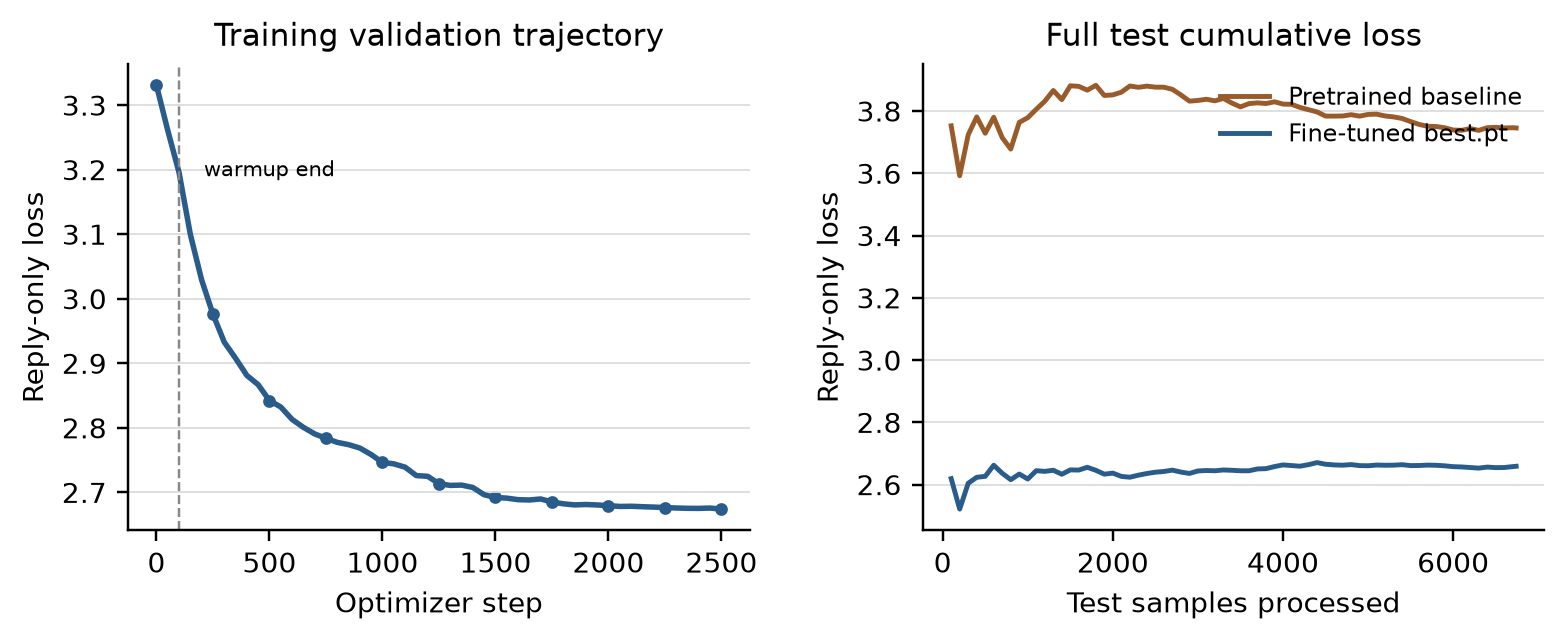
\includegraphics[width=\textwidth]{figures/training_and_test_loss.png}
\caption{左：2500-step run 全过程的 validation monitoring右：两个模型遍历完整 test split 时的 cumulative reply-only loss}
\label{fig:training-test-loss}
\end{figure}

\subsection{完整 held-out test evaluation}

最终 comparison 独立于由 40 条 samples 构成的 validation monitoring subset，两个 W\&B evaluation runs 按照相同的 deterministic order 遍历全部 6740 条 held-out test samples，每个 run 的 batch size 均为 2，在相同的 107,825 个 supervised reply tokens 上累计 loss，并在 \texttt{model.eval()} 与 \texttt{torch.no\_grad()} 下执行，不更新任何 parameter。

\begin{table}[htbp]
\centering
\caption{完整 test split 对比}
\label{tab:test-results}
\begin{tabular}{lrr}
\toprule
Model & Test loss & Perplexity\\
\midrule
Pretrained DialoGPT-small baseline & 3.745823 & 42.343856\\
Fine-tuned \texttt{best.pt}, step 2500 & 2.659185 & 14.284649\\
\bottomrule
\end{tabular}
\end{table}

Fine-tuning 使 test loss 降低 1.086638，相对降幅为 29.01\%，同时 perplexity 下降 66.27\%。图~\ref{fig:training-test-loss} 中的 cumulative curves 在整个 test traversal 过程中始终分离，并最终收敛到表~\ref{tab:test-results} 所列数值。完整 held-out split 上的一致结果表明，测得的改善并不局限于 checkpoint monitoring 使用的小型 validation subset。对应的 W\&B run IDs 分别为 baseline 的 \texttt{nj6qn3m9} 与 \texttt{best.pt} 的 \texttt{gk54iku3}。Evaluation progress 记录为 \texttt{evaluation/batch}、\texttt{evaluation/samples} 和 \texttt{evaluation/tokens}；cumulative result metrics 为 \texttt{test/loss} 与 \texttt{test/perplexity}，默认以 processed samples 作为 step coordinate。

\subsection{Fixed-prompt baseline comparison}

五个指定 prompts 均使用 seed 1337、maximum 50 new tokens、temperature 0.75、top-$k$ 50 与 repetition penalty 1.1 生成。Baseline 与 fine-tuned generation 使用相同的手写 sampling path，并在运行每个模型前将 CPU generator 重置为相同 seed，以下 outputs 均为原始记录。

\subsubsection*{Prompt: Hello!}
\begin{quote}\small
\textbf{Baseline.} Welcome to the subreddit . It's me , and it feels good ! u flappy bird cat also likes pineapple on pizza : 3 Mwahahahaha Edit just kidding I thought you were a girl ... but nice catch anyways .. haha xD g

\textbf{Fine-tuned.} Hi , Paul ! I'd like to see this picture please . It's really fresh . How much is it ?
\end{quote}

\subsubsection*{Prompt: How are you today?}
\begin{quote}\small
\textbf{Baseline.} That's very interesting , and something I've not seen discussed around here before . Does the difference in sleep have any relevance to whether or no REM meds should be used ? Thanks ! :D lt 3 edit jinxed it .. bye again

\textbf{Fine-tuned.} I'm fine.Thank ' s for asking . How's your day ? What did she say to you , Mr Li or Ms li about the show last night with her husband again and who else is going on vacation from New York tonight at noon morning
\end{quote}

\subsubsection*{Prompt: What do you like to do?}
\begin{quote}\small
\textbf{Baseline.} I'm curious , what kind of stuff ? Just social things are fine . We usually don't have too hard a say in these types if we meet up again on Friday evening ! :D Hope it goes well though ... lt 3hugs c

\textbf{Fine-tuned.} I want a travel agent and I ’ Ve always liked American Airlines . And with this company , there's no better choice than B\& T in the same region as Air India or Malaysian airlines ? So why are they different now that it is popular
\end{quote}

\subsubsection*{Prompt: I'm feeling a little sad.}
\begin{quote}\small
\textbf{Baseline.} So ... where are we all going ? ! Edit : thanks for the gold kind stranger . I can't wait to go there with my family and eat some nice pizza again when season 7 rolls around .. sips champagne yep , that's me too

\textbf{Fine-tuned.} How about you ? What are your health problems in the meantime on this boat again , and what's changed over time with all that good news . Good luck anyway ! I hope someone will help me find out some answers to those of my questions . That
\end{quote}

\subsubsection*{Prompt: Tell me something interesting.}
\begin{quote}\small
\textbf{Baseline.} Well , not the same as my name . That's a bummer too man .. but I'm going with it anyways ... just felt like sharing you guys had so much in common ! Lol ? :P P Anyway happy hunting XD D: lt

\textbf{Fine-tuned.} Do you have a picture of our office ? How much are we talking about for that photo ? I think its worth \$ 50 . Will it be safe to show off the house while leaving or is this too expensive at best in order make sure there's
\end{quote}

\subsection{验收结论}

五个 fine-tuned outputs 均为非空、可解码的 English-like suffixes，且没有任何一个等于其 normalized prompt；Fine-tuned model 的 full-test loss 也严格低于 pretrained baseline，因此同时满足本项目定义的 quantitative criterion 与 minimum generation checks；然而，这些 examples 仍揭示了明显的 qualitative limitation：回复的 relevance 与 long-range coherence 并不稳定，尤其是在 response 接近 50-token cap 时。Loss reduction 证明 DailyDialog next-token modeling 得到改善，但不代表模型能够始终生成可靠且上下文精确的对话。

\end{document}
